% =====================================================================
% Clase -- Geometría 5° -- Trimestre I -- Semana 03
% Sesión 002 (lun 14 sep., 06:55, 55 min)
% Tema: Sistemas de referencia
% Subtema: De la posición relativa a la cuadrícula: filas y columnas
% Hilo conductor del trimestre I: «Cali, mi ciudad»
% Tema 1 de la guía: Sistemas de referencia (tema:referencia)
% Material del docente (no se entrega a los estudiantes).
% =====================================================================
\documentclass[11pt]{article}
\makeatletter\def\input@path{{../../../../../plantillas/estilo/}}\makeatother
\usepackage{mmcantillo}
\guiadelestudiante{../../guia-didactica/guia-periodo-I-ubicacion}

\tipodocumento{Clase}
\asignatura{Geometría}
\titulo{Semana 3: de «al lado de la ventana» a la cuadrícula}
\grado{5°}
\periodo{I}

% DBA: matematicas grado 5 · DBA 7 — Resuelve y propone situaciones en las que es necesario
% describir y localizar la posición y la trayectoria de un objeto con referencia al plano
% cartesiano. Evidencias de esta sesión: «Interpreta los elementos de un sistema de
% referencia» y «Representa en forma gráfica y simbólica la localización de un objeto».

\begin{document}

\encabezado*

\begin{center}
{\renewcommand{\arraystretch}{1.3}
\begin{tabularx}{\linewidth}{@{}l l l X l@{}}
  \toprule
  \textbf{Sesión} & \textbf{Fecha} & \textbf{Min} & \textbf{Subtema} & \textbf{Entregables}\\
  \midrule
  002 & lun 14 sep., 06:55 & 55 & De la posición relativa a la cuadrícula: filas y columnas
      & Tarea 1 (para el lun 21 sep.)\\
  \bottomrule
\end{tabularx}}
\end{center}

Esta sesión recoge el plano del salón que los estudiantes dibujaron la semana pasada y lo
convierte en un sistema de referencia con filas y columnas. Es el primer paso del camino que
termina en el plano cartesiano (sesiones 004 y 005) y abre el hilo del trimestre: \emph{Cali,
mi ciudad}, apoyado en algo que los estudiantes ya usan sin darse cuenta —las direcciones de
la ciudad se dan con calles y carreras, que forman una cuadrícula.
Referencia: \refguia{tema:referencia}.

% ---------------------------------------------------------------------
\seccion{Sesión 002 — lunes 14 de septiembre · 06:55 · 55 min}

\textbf{Objetivo.} Describir la posición de un objeto usando un sistema de referencia de
filas y columnas, y escribirla de forma abreviada, en lugar de describirla con expresiones
relativas («al lado de», «detrás de»).

\textbf{Materiales.} Tablero; el cuaderno con el plano del salón de la semana pasada; hojas
cuadriculadas; regla.

\begin{center}
{\renewcommand{\arraystretch}{1.3}
\begin{tabularx}{\linewidth}{@{}l l X@{}}
  \toprule
  \textbf{Momento} & \textbf{Min} & \textbf{Actividad}\\
  \midrule
  Enganche & 0--8 & Retomar el plano del salón de la semana pasada. Pedirle a un estudiante
    que explique dónde se sienta \emph{sin señalar con el dedo y sin decir nombres de
    compañeros}. Anotar en el tablero las expresiones que use («al lado de la ventana»,
    «detrás de»). Pregunta: «si llega un estudiante nuevo mañana, ¿con estas indicaciones
    encontraría el puesto?»\\
  Explicación & 8--20 & Introducir el término \textbf{sistema de referencia}: un acuerdo
    fijo para decir dónde está algo. Dibujar en el tablero la cuadrícula del salón: las
    \textbf{filas} se nombran con letras ($A$ a $D$), empezando por la más cercana al
    tablero, y las \textbf{columnas} con números ($1$ a $5$), de izquierda a derecha mirando
    al tablero. Escribir la posición abreviada como un par:
    $(B,3)$ se lee «fila $B$, columna $3$». Insistir en el orden acordado: primero la fila,
    después la columna; si se invierte, se llega a otro puesto.\\
  Práctica guiada & 20--38 & Con la cuadrícula del salón (ver figura): la docente dice una
    posición y los estudiantes escriben quién o qué está ahí; luego al revés. Después, en
    parejas, cada estudiante escribe en el cuaderno su propia posición y la de dos
    compañeros.\\
  Cali, mi ciudad & 38--50 & Mostrar el plano del barrio (ver figura) y contar que Cali está
    organizada así: las \textbf{calles} van en un sentido y las \textbf{carreras} en el otro,
    y por eso una dirección se da con dos números («Calle 5 con Carrera 39»). Preguntar:
    «¿qué hay en la Calle 2 con Carrera 3?», «¿cómo le explicarías a alguien que acaba de
    llegar a Cali dónde queda el parque?»\\
  Cierre y tarea & 50--55 & Cerrar con la idea clave: \emph{dos datos bastan para ubicar un
    punto, si antes acordamos desde dónde se cuenta}. Asignar la Tarea 1, para el lunes 21 de
    septiembre.\\
  \bottomrule
\end{tabularx}}
\end{center}

\textbf{Cuadrícula del salón (para copiar en el tablero).}

\begin{center}
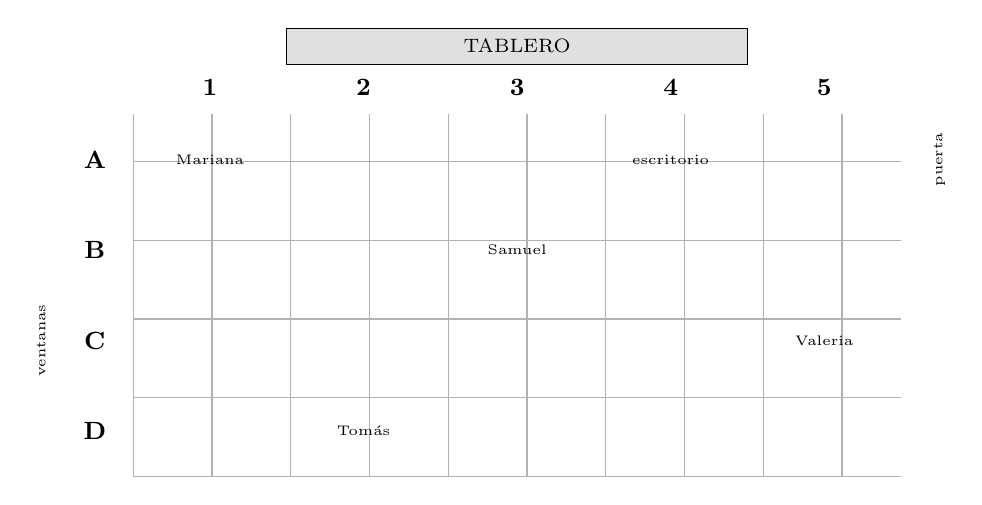
\begin{tikzpicture}[x=1.95cm, y=1.15cm, font=\tiny]
  \draw[gray!60] (0,0) grid (5,4);
  \foreach \x/\n in {0.5/1, 1.5/2, 2.5/3, 3.5/4, 4.5/5}
    \node[font=\small\bfseries] at (\x,4.3) {\n};
  \foreach \y/\l in {3.5/A, 2.5/B, 1.5/C, 0.5/D}
    \node[font=\small\bfseries] at (-0.25,\y) {\l};
  \draw[fill=black!12] (1,4.55) rectangle (4,4.95);
  \node[font=\scriptsize] at (2.5,4.75) {TABLERO};
  \node[align=center] at (0.5,3.5) {Mariana};
  \node[align=center] at (2.5,2.5) {Samuel};
  \node[align=center] at (4.5,1.5) {Valeria};
  \node[align=center] at (1.5,0.5) {Tomás};
  \node[align=center] at (3.5,3.5) {escritorio};
  \node[rotate=90] at (5.25,3.5) {puerta};
  \node[rotate=90] at (-0.6,1.5) {ventanas};
\end{tikzpicture}
\end{center}

\textbf{Respuestas de la práctica guiada.} Mariana está en $(A,1)$; Samuel en $(B,3)$;
Valeria en $(C,5)$; Tomás en $(D,2)$; el escritorio de la docente, en $(A,4)$. La puerta
queda junto a la fila $A$, al lado de la columna 5; las ventanas, al lado de la fila $C$.

\begin{nota}
Si alguien dice «Samuel está en $(3,B)$», no lo corrijas como un error de cálculo: es el
momento de mostrar por qué hace falta un \emph{acuerdo}. Pregunta al grupo qué puesto
señalaría alguien que leyera ese par al revés. El acuerdo de esta clase —primero la fila,
después la columna— se mantiene todo el trimestre.
\end{nota}

\textbf{Plano del barrio (Cali, mi ciudad).}

\begin{center}
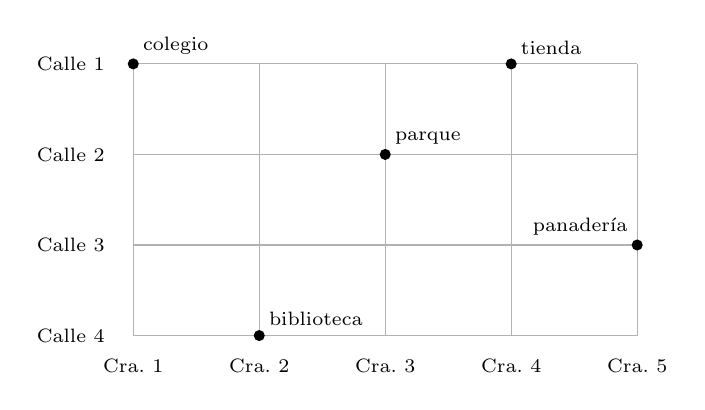
\begin{tikzpicture}[x=1.6cm, y=1.15cm, font=\scriptsize]
  \foreach \x in {0,1,2,3,4} \draw[gray!60] (\x,0) -- (\x,3);
  \foreach \y in {0,1,2,3} \draw[gray!60] (0,\y) -- (4,\y);
  \foreach \x/\n in {0/1, 1/2, 2/3, 3/4, 4/5}
    \node[anchor=north] at (\x,-0.15) {Cra.~\n};
  \foreach \y/\n in {0/4, 1/3, 2/2, 3/1}
    \node[anchor=east] at (-0.15,\y) {Calle~\n};
  \fill (0,3) circle (2pt); \node[anchor=south west] at (0,3) {colegio};
  \fill (3,3) circle (2pt); \node[anchor=south west] at (3,3) {tienda};
  \fill (2,2) circle (2pt); \node[anchor=south west] at (2,2) {parque};
  \fill (4,1) circle (2pt); \node[anchor=south east] at (4,1) {panadería};
  \fill (1,0) circle (2pt); \node[anchor=south west] at (1,0) {biblioteca};
\end{tikzpicture}
\end{center}

\textbf{Respuestas del plano del barrio.} En la Calle 2 con Carrera 3 está el parque; el
colegio queda en la Calle 1 con Carrera 1; la tienda, en la Calle 1 con Carrera 4; la
panadería, en la Calle 3 con Carrera 5; la biblioteca, en la Calle 4 con Carrera 2.

\begin{nota}
No introduzcas todavía las palabras «plano cartesiano», «eje» ni «coordenadas», ni uses
números para las filas: eso llega en las sesiones 004 y 005, y la fuerza de esas clases está
en que los estudiantes lleguen pidiendo un sistema más cómodo. Aquí basta con filas, columnas
y el par ordenado. Los puntos cardinales entran en la sesión 003.
\end{nota}

\end{document}
